\documentclass[12 pt]{article}
\usepackage[margin = 1.0in, letterpaper]{geometry}
\usepackage{graphicx}
\usepackage{amsfonts, amsmath}
\usepackage{float}

\begin{document}

\title{Hydrogen Emission Lines and the Orion-Eridanus SuperBubble}
\author{Eduardo Herrera}

\maketitle
  
\begin{abstract}
    Examining the emission of Hydrogen (the H1 line) and using the
Leushner telescope we were able to take data for about  points from
the Orion-Eridanus SuperBubble. Using the calibrated data sets for these points,
an image of the Super-Bubble could be resolved, albeit at about half the
resolution originally intended due to hardware and organization problems
leading to lack of time. From an analyzation
of this image we can see the different column densities of the Hydrogen
where a bubble structure confirms that it has been expanding
and we can also see the feautures of the bubble such as thicker clouds of
Hydrogen gas around the circumference of the bubble (around 7 $cm^2$)
present there whereas near the center of the bubble a thinner
layer of gas is observed as evidenced by the color intensity of the column densities calculated for the
bubble. . 
\end{abstract}

\section*{Introduction}
The Orion Super-Bubble is the remnant of a supernova and the stellar
winds that resulted from it. Due to this explosion, a shock
from the original supernova pushed dust and gas outward. As a
result of there is an empty space that is surrounded by a wall of gas previously
mentioned. The surface of this bubble has neutral gas and contains some
features that indicate that there is ionized gas that emits
synchrotron radiation.  Hydrogen emission is critical to revealing the
structure of our Bubble, because the 21 cm line for Hydrogen can easily
pass through the interstellar medium present between the Bubble and the
telescope, additionally, the vast amount of hydrogen present in the
Universe makes this method of observing objects the most preffered. For this project, the Orion
Super-Bubble, covers latitudes from -10 to -70 degress in galactic
coordinates and longitude of 160 to 220 degrees, covering a total of
2800 degrees of sky.
\begin{figure}[H]
\centering
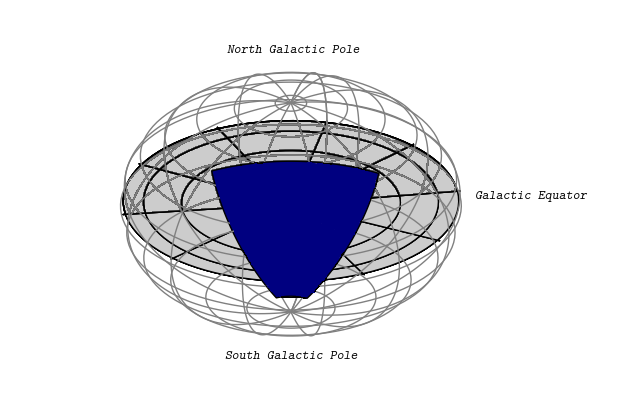
\includegraphics[scale=0.75]{cooords.png}
\caption{A 3D plot of the total amount of sky that the Orion SuperBubble
  covered that in turn could be observed
  by the Leuschner telescope at 2 degree spacings. A 2800 degree area in the sky; taking up
  about a fifth of the sky this meant the possibility of taking up to
  700 pointings. }
\label{galaccooords}
\end{figure}
 Due to time constraints caused by the class's groups
(procrastination), not all of the 700 pointings could be covered. Results of our observations
include a half resolution image of the Super-Bubble. The following section discusses the
observer for all of our data, followed by the process by which the raw
data was calibrated to produce a final spectrum for the Hydrogen line
observed. Then a section on the techniques used to image the SuperBubble
and an analyzation of the physical features of the Bubble follows.   
\section*{The Leuschner Telescope}
In regards to the telescope, we used the Leuschner telescope, with a dish
diameter of 4.5 meters. Since we are observing the 21 cm hydrogen
profile, then the resolution of the dish is $\theta =
\frac{\lambda}{D}$, $\theta = \frac{.21m}{3.6m} = .0583$. \par
Present between the galactic latitudes of -10 to -70 degrees and 160 to 220
degrees longitude, the Orion Super-Bubble spans an area of 2800  square
degrees originally it was planned to take measurements at points 2
degrees apart so this meant making 700 pointings for which we would need
data. Hardware issues on the telescope as well as a lack of organization
could only allow about half of these pointings. 
\subsection*{How Information Reaches the Telescope}
When the telescope is pointed to a source, photons from the source will
get to the telescope and be reflected by the dish and into its
detector. The telescope measures the intensity of the object, meaning
that a time interval between observations over some area of the sky. In
tensity is measured by Energy per time per area. The intensity at which
the telescope gathers data is $I(\nu) =\frac{2k_{B}T}{\lambda^2}$
because $\frac{h\nu}{k_{B}T} << 1$. Our hydrogen, when excited, is at a
relatively high temperature compared to other things reacting to
heat. One important aspect of specific intensity when observing a source
is that $I(\nu)$ is constant along the ray's path. This has the
consequence that the specific intensity of the 'lens' of the telescope
is equal to that of the source, independent of distance, $I_{scope} =
I_{source}$. Since the sources in the sky have some differences in their
frequencies there is a temperature dependence as well, so we can then
define intensity in terms of a temperature, a \textit{brightness
  temperature}, $T_{B}= \frac{I(\nu)}{2k_{B}}\lambda^2$ but in general
this temperature is not equal to the temperature of the source, the
brightness temperature merely characterizes the object from its emitted
intensity. Another temperature to take into account is the
\textit{antenna temperature}, which when the telescope's beam is larger
than the object it attempts to take measurements from,  is defined as
$T_{v}(\nu)=T_{B}(\nu)(\frac{\Omega_{source}}{\Omega_{source}+\Omega_{beam}})$ 
\subsection*{Coordinates and Pointing Strategy}
Again, the use of rotation matrices was key to get the telescope to
point at the appropriate sources, but fortunately compared to the last
lab, we only had to account (on top of the previous code from the last
lab) for galactic coordinates which treats the sun as the origin of its
polar coordinate system, a primary direction toward the center
of our own galaxy, and its plane in line with the plane of our own
galaxy, this system makes finding objects within our own galaxy easier. \par
In order to keep as much time as possible for the observation of our
points, we chose to use the rastering strategy. This involves the
telescope sweeping across the sky stopping at its designated observing
points when necessary. When the script was at the end of a sweep it
would simply go down to the next point below the one it had just taken
data for instead of sweeping back over (much like a typewritter). This would then save time for
taking on more points. \par
On a more technical level, we needed to choose two local oscillation
(LO) frequencies, one that was at 1272.2 MHz and the other that was
shifted off by 4 Mhz at 1268.2 MHz The reason we chose these values was
to alias the Hydrogen line making it easier to discern it from the data
when we opened it. The reason we shift this frequency is
to use the noise diode onboard the telescope to increase the amplitude
of our measurements, which are weak sources for the most part. The noise
measurements are made for both times when the LO frequency, but because
of the noise, there will be large spikes in the data mostly due to the
first amplifier present on the telescope, before anything can be done,
it must somehow get cleaned.  

\section*{Treating the Raw Data}
In calibrating our raw data, we see 4 continuum spectra
with spikes that present the hydrogen line. But this data is riddled
with spikes as a result of the amplifier making a lot of noise in the
data, making any attempt to add the spectra worthless since the original
data with the hydrogen line could be wiped out when added and averaged
across other smaples. To get rid of these samples, a box-car average
over this data is needed to get rid of the spikes and have some good
data to work with for the later step of convolvement into a final
spectrum for each data set. Instead of a mean, we take a median between
every few points making sure the bin does not exceed the width of the
observed Hydrogen spike, otherwise the box car average would interpret
the spike as the noise we are trying to measure and flatten it out. As a
result of using a good cleaning code is, the following. 
\begin{figure}[H]
\centering
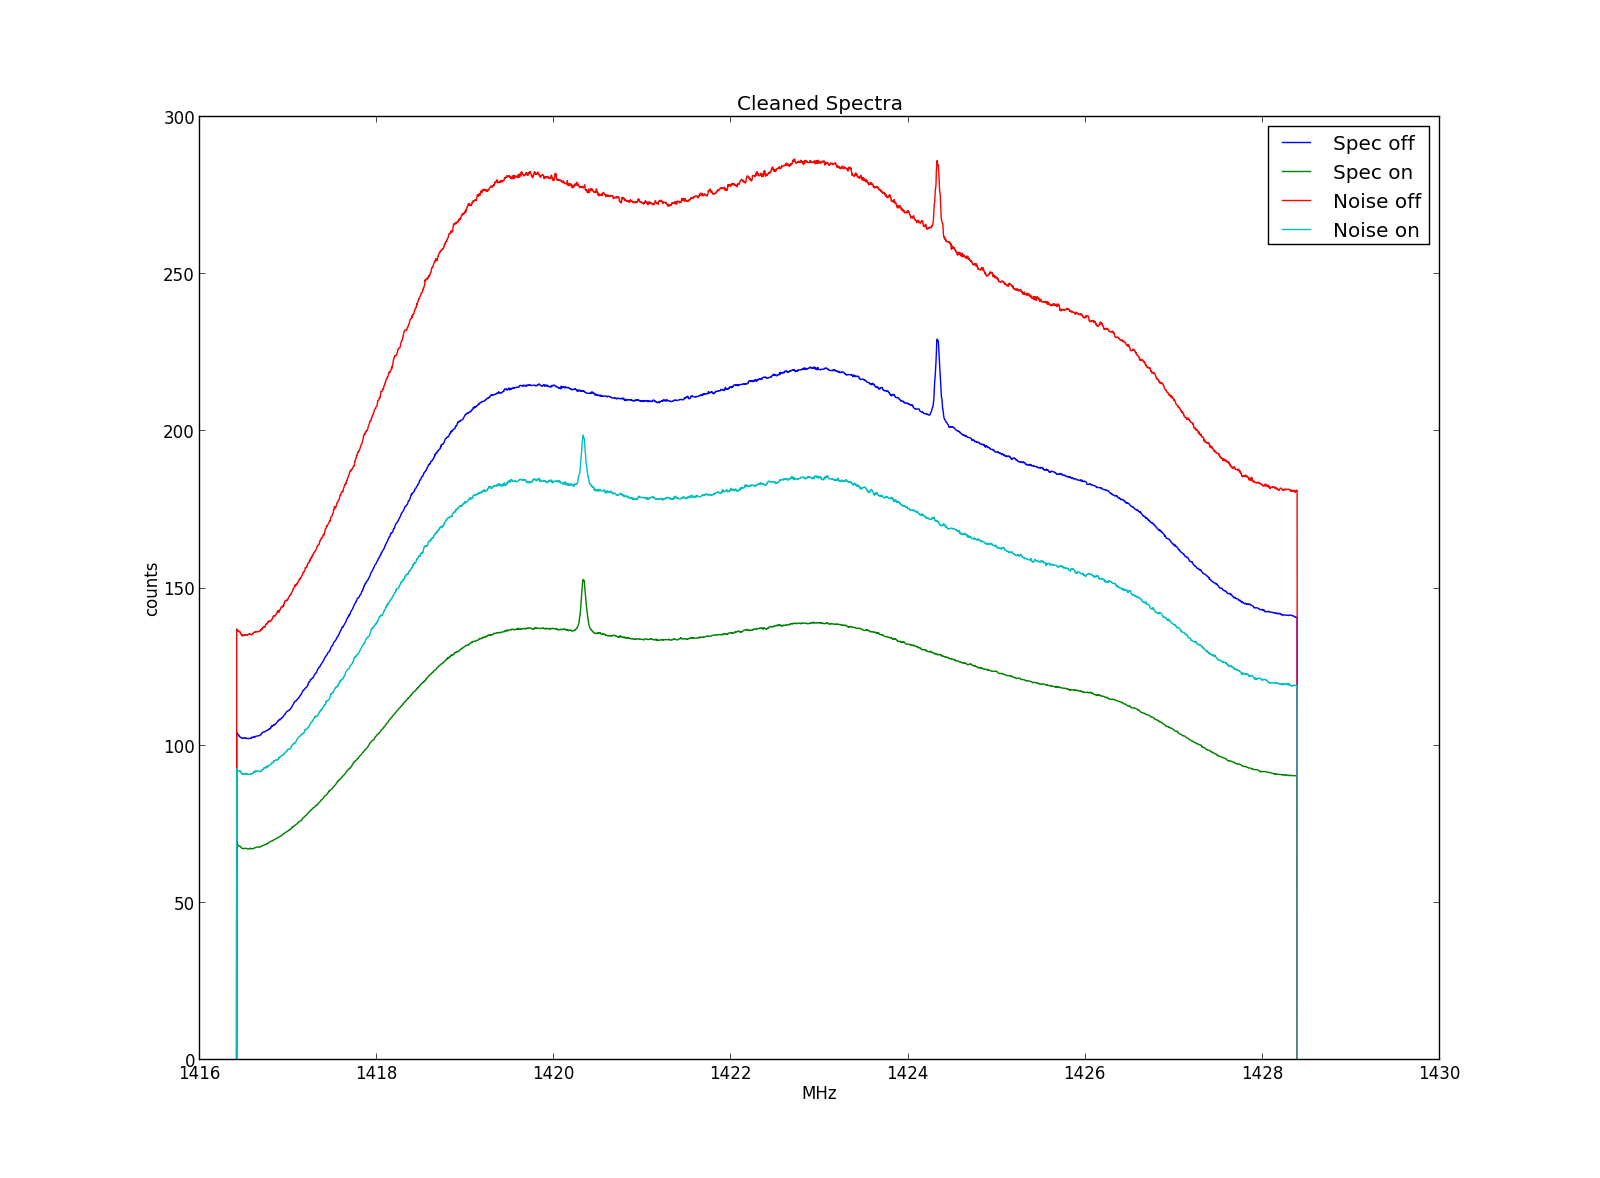
\includegraphics[scale = 0.45]{cleandata.png}
\caption{after using a reasonable size for the bin to take the median,
  we get a spectrum that cuts down significantly on noise, to clarify on
lalbels, spec off and on refer to the LO frequencies being on the value
we originally chose and shifted off, respectively. As for noise off and
on, both mean that the noise diode was turned on for both cases of the
LO frequency being either on or off target,  no noise diode was ever
turned off.}
\label{cleandata}
\end{figure}
Regarding the calibration time, the Bubble only required about 22
seconds of calibration time, $\tau$,  at first it may seem that we need
more than that to get a higher resolution for an image. But a look at
the radiometer equation shows
\begin{equation}
  \sigma_{T}= \frac{T_{sys}}{sqrt(B\tau)}
\end{equation}
The important thing to note is that when we measure with the noise diode
on, to achieve the same temperature brightness resolution, we do not
need to integrate as long since B, the bandwidth takes care of the noise
measurement made, now instead of worrying about a bin to bin basis, we
use the whole 12 MHz available to us so that our integration time is
lowered to meet the same brightness temperature resolution. This should
also lower the noise level as we do increase integration time by an
inverse factor of $\sqrt(\tau)$.
\subsection*{Calibration}
With cleaned data, a calibrated spectra is now possible to get. Because
of the noise diode is there to build up the calibrated
hydrogen line; to give both the original LO and the shifted LO an
increased amplitude. Because we were able to invest the time, our group
went for the 'cool' method of getting calibrated spectra out. First, we
may assume that the Temperature of the noise diode $T_{noise} = 100$ is
a constant. Next we create a Y factor for both the LO frequencies
consisting of the sum of noise measurements and on spectrum
measurements, which also looks similar for the off measurement
frequencies. What the Y factor is though, is the our noise on
measurement, which is equal to the temperature of the system plus the
temperature created in the telescope by the noise diode, so that
$Y_{on}=1+\frac{T_n}{T_s}$ and by analogy the o Y factor for the off
measurement is similar to the previous equation. With these Y factors,
we can then solve for the temperature of the system for both the on and
off measurements. One additional thing is the ratio of the gains,  equal
to the division of the sums of the spectrum of the measurements with the
two LO frequencies. With this we must re-define the spectrum
measurements by multiplying the original spectrum measurements by the
gain ratio. Here we divide the new spectrum measurements while not
dividing out the hydrogen line feature, this allows for the flattening
of the noise measurements while keeping the structure of the hydrogen
lines. Additionally we must add them together and divide by two to get
the average of the summed hydrogen lines, and thus we get a calibrated
spectrum as shown. 
\begin{figure}[H]
\centering
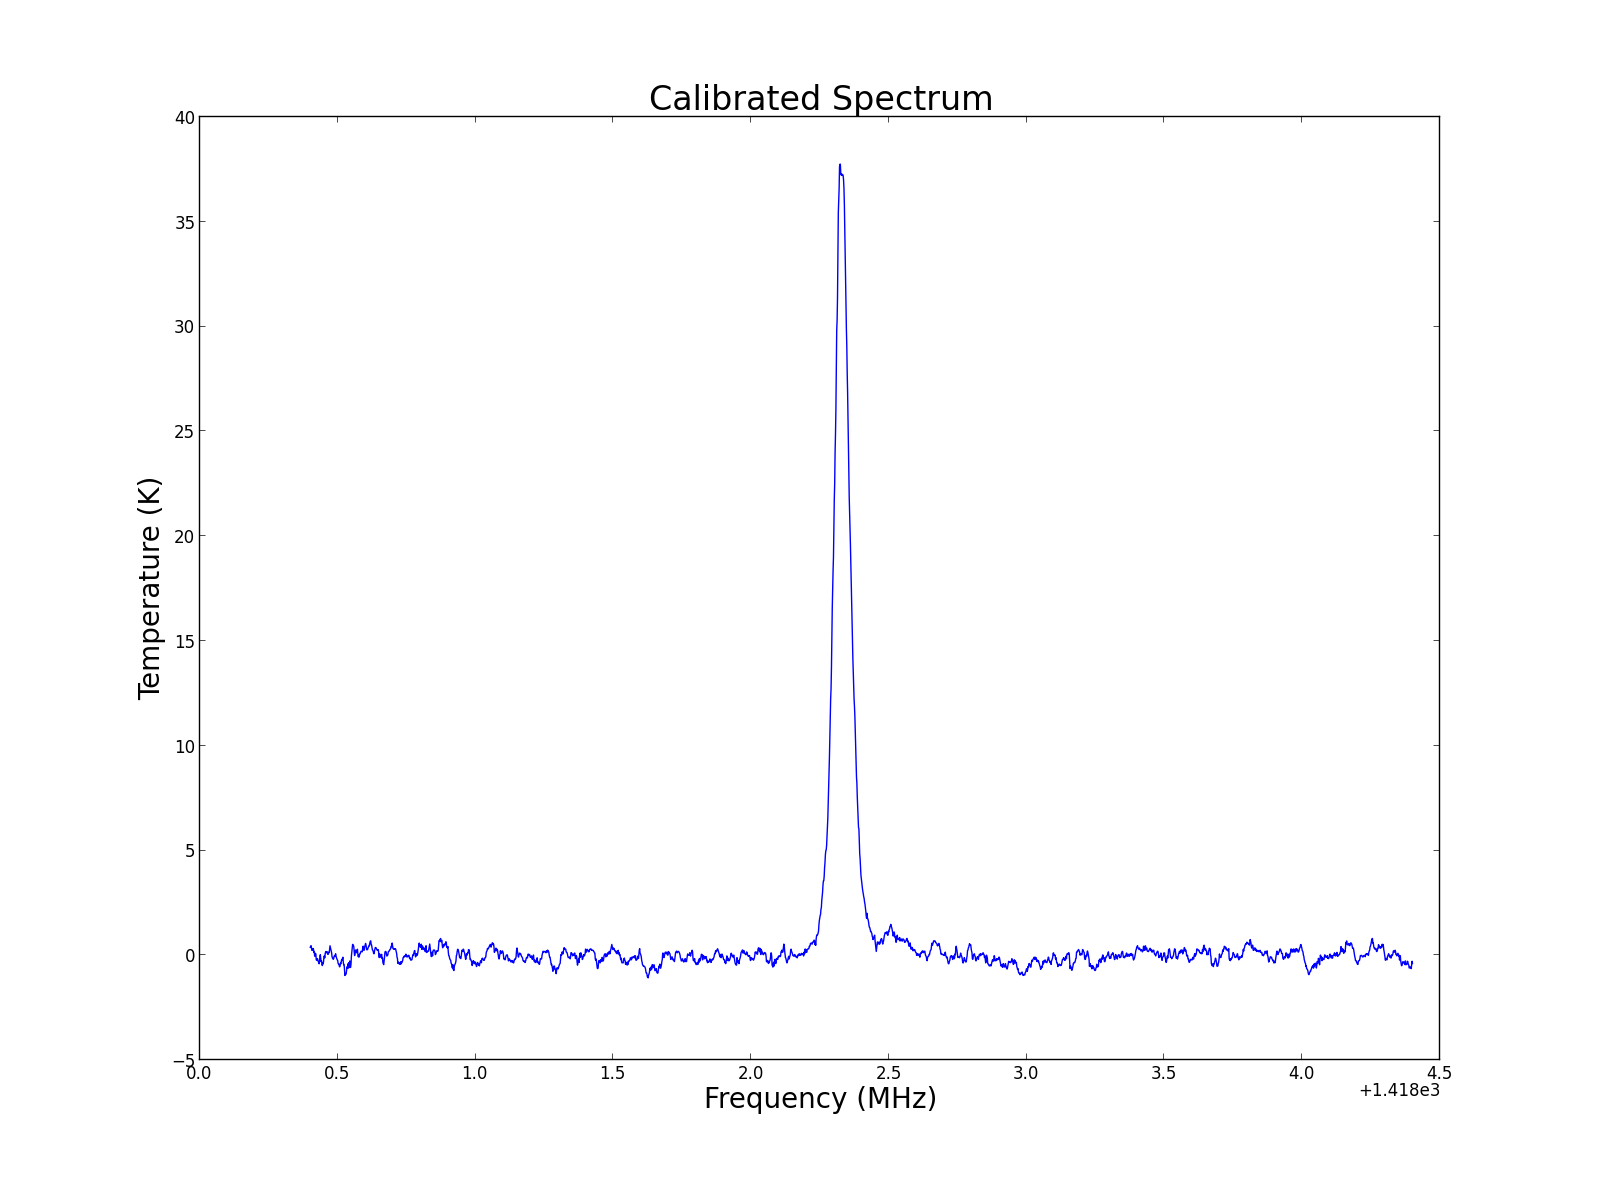
\includegraphics[scale=0.45]{calibspect.png}
\caption{An example of a calibrated spectrum for one data point in the
  Orion Super bubble, it looks like a sharp spike, most look like this,
  but there are others that exhibit the feature of a double spike in the
  calibrated data, this is telling of seeing contributions from both the
  front and the back of the bubble; a doppler shift of the expanding
  bubble, showing both a red shifted and blue shifted spectrum on the
  same line. As for this more common spectrum, a single spike may come
  from the edges of the bubble where from our point of view the gas is
  expanding perpendicularly, no shift.}
\label{calibspect}
\end{figure} 

\section*{Imaging the SuperBubble}
After all of the individual data points had been calibrated and 
saved to one file,  there still remained to plot the image across the
area we had abserved it from in galactic coordinates. To achieve this,
we needed to take the data forms of the file; longitude, latitude, and
the spectrum. And manipulate the data points so that they would be put
on a 1000 by 1000 resolution image. Not only that but since we only have
a few points to work with, we would have to interpolate all points with
one another by using a gaussian that depended on the points themselves
and some arbitrary number of pixels for which the gaussian would
convolute over. First by creating two grids, one for which your points
will fall into the image and the other for the weights that the gaussian
will be convolved with. To plot the points,  an array of zeros must be
implemented as well with the weights, for every latitude coordinate,
set the weights equal to one for points that will otherwise be
empty. After populating the other points with your data,  then you have
a grid with your points surrounded by what seems a sea of blue. The
gaussian is set to take in the points that happen to be there so that
points containing data points will be more convolved than areas barren
with points. After compiling the image one must take note that the axis
for the longitude are not exactly accurate,  since we are in polar
coordinates,  the vertical axis must be adapted to fit the curvature. 

\begin{figure}[H]
\centering
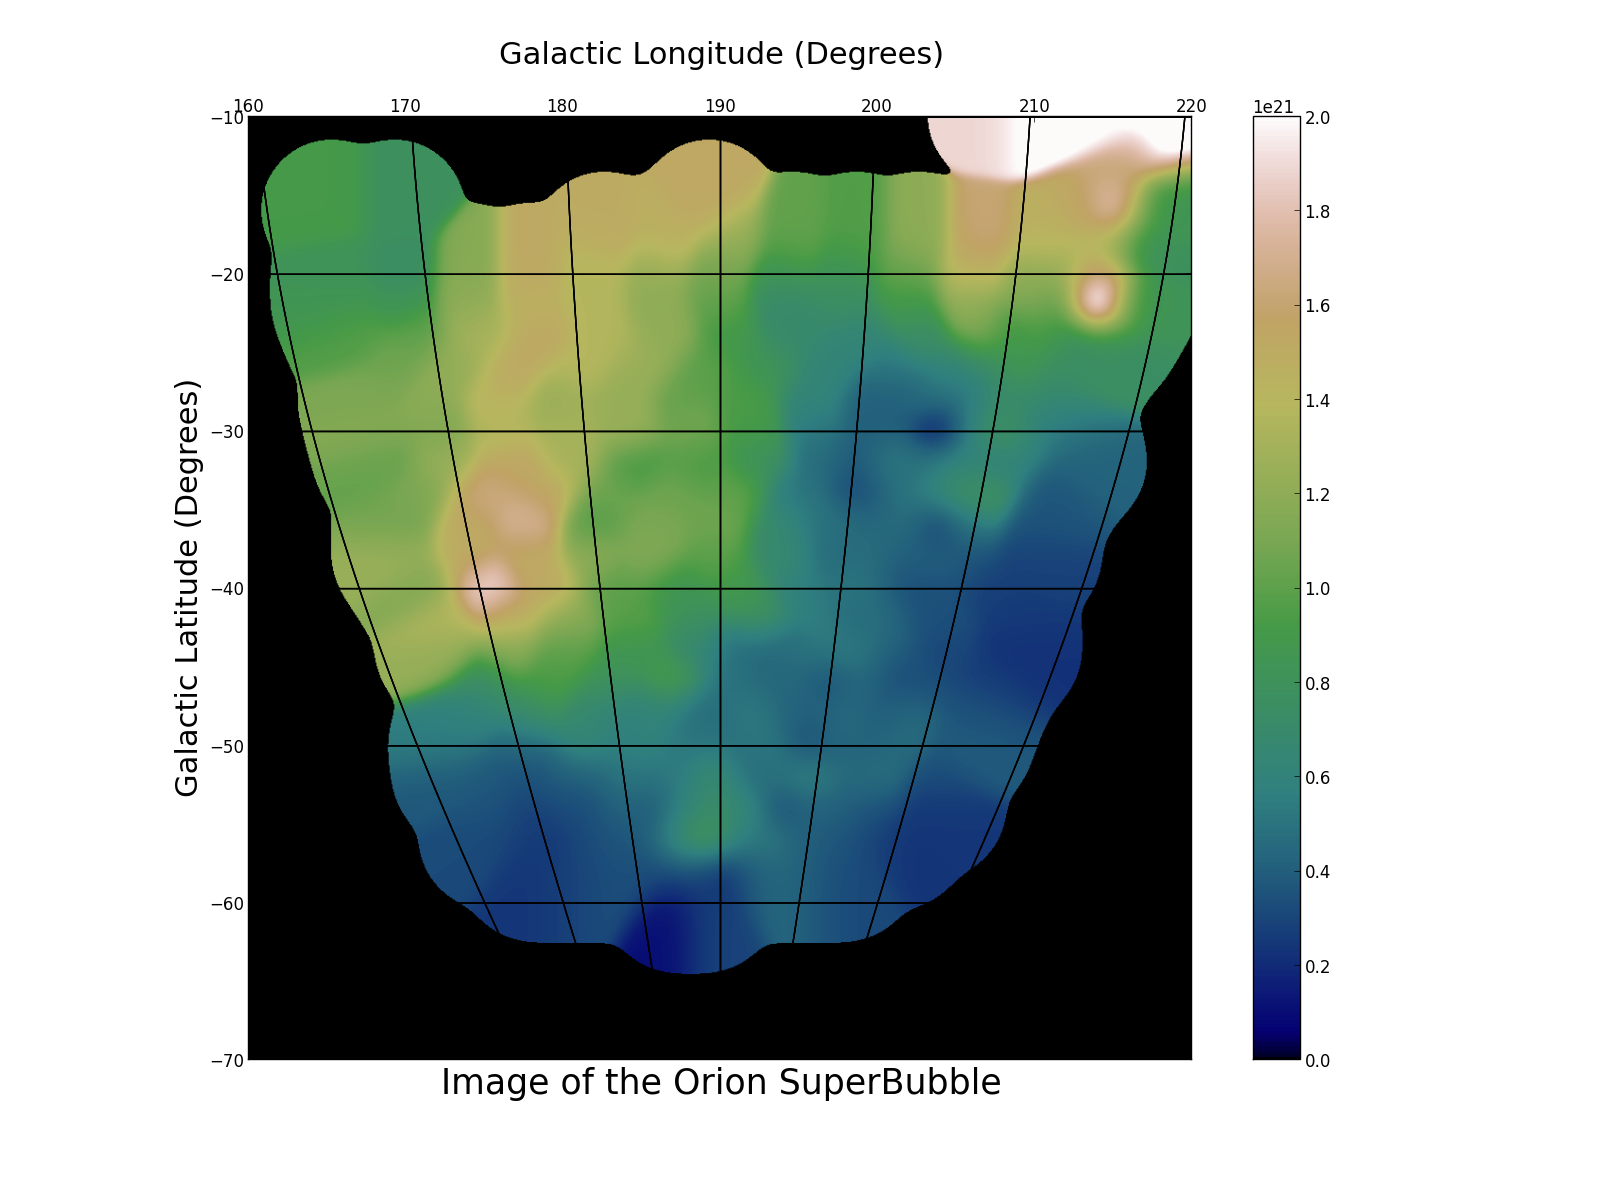
\includegraphics[scale=.45]{bubbleimage.png}
\caption{The Final image of the Orion superbubble consistent with other
  researchers, a hollower area inside with thick walls of hydrogen
  surrounding the bubble}
\label{bubble}
\end{figure}

Comparing the above image to the one taken by 'The Orion OB1
association' headed by A.G.A. Brown, D. Hartmann and W.B. Burton from
the Netherlands,  we see that they have a wider area of observation with
larger resolution. Flipping their image and concentrating on the area
corresponding to ours. 

\begin{figure}[H]
\centering
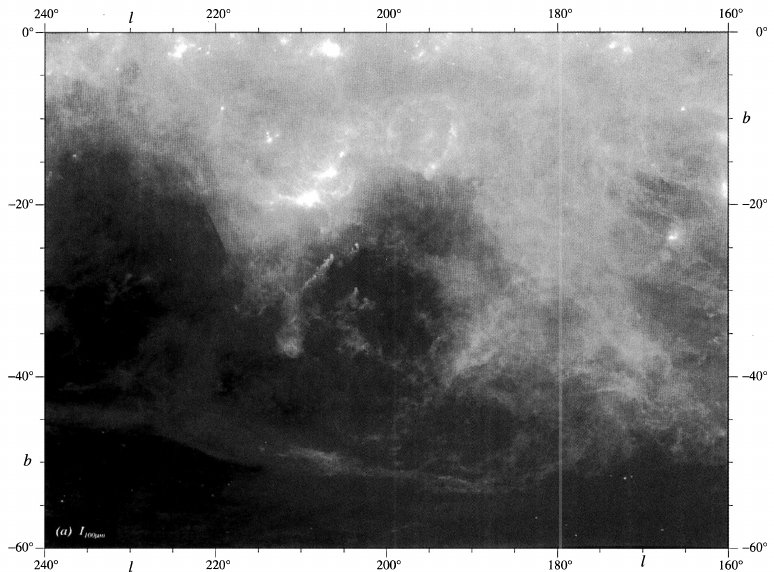
\includegraphics[scale=.6]{actual orion.png}
\caption{a comparison with an image taken by A.G.A. Brown et al.: 'The
  Orion-Eridanus Bubble'. As we can see if this image were flipped and
  concentrated around latitude -30 and -200 degrees, we can see that our
image matches up well at least in shape, and we can see a bubble
structure surrounded by gas.}
\label{actualorion}
\end{figure}

\section*{The Bubble's Column Density}
The column density tells us how much gas there is per square centimeter 
to have calculated we needed to have every element of the spoectrum be
multiplied by $1.8*10^{18}*12000khz/(8129 channels*4.73khz)$ to give us
the column density on order of one to two $1e21 cm^{-2}$.
\section{Conclusion}
We can see that the bubble has a lower density around the coordinates of
-35 latitude and 200 longitude,  as does the the diagram from
A.G.A. Brown. Even with less than half resolution, we were still able to
make an image that has evidence of a bubble in the middle. 

\section*{Acknowledgements}
A.G.A. Brown et al.: 'The
  Orion-Eridanus Bubble' pg 14

\end{document}